%!TEX root = ../intro.tex
%******************************
%	 Bayesian approaches
%*****************************

\section{Bayesian approaches to model scRNAseq data}

In the last decade, an array of tools to process and analyse scRNA-Seq data has been developed. These methods include preliminary tools for data acquisition (e.g.~alignment, de-duplication, quantification), data filtering (e.g.~quality control, normalization, imputation), cell labelling (e.g.~clustering, classification, ordering) and gene-level analysis (e.g.~differential expression, detection of expression patterns) \citep{Zappia2018}. Extensive comparisons of these methods have been done in details depending on the type of analysis that need to be performed \citep{Saelens2018, Soneson2018}. At this point, I want to focus on Bayesian methods that were developed to estimate posterior distributions for model parameters to propagate uncertainty into downstream analysis. \\

\subsection{The basics of Bayesian inference}

The main difference between classical and Bayesian inference is the distributional assumption of the model parameters. While in classical inference, model parameters represent an fixed but unknown value, Bayesian approaches treat parameters as random variables to incorporate the uncertainty of parameter estimation \citep{Bernardo2003}. The aim of Bayesian inference is to find a \emph{posterior distribution} that captures the uncertainty of the model parameter $\omega$. Prior believes about the distribution of $\omega$ are summarized in form of a \emph{prior distribution} $\pi(\omega)$. Once the data $D$ is observed, the prior distribution $\pi^*(\omega|D)$  is updated to form the posterior distribution of the model parameter $\omega$. This is a simplified explanation of the Bayes Theorem \cite{Canton1763}:

\begin{equation} \label{eq0:Bayes_theorem}
\pi^*(\omega|D,\cdot)=\frac{L(D|\omega)\pi(\omega)}{L_\omega(D)}.
\end{equation}

Here, $L(D|\omega)$ is the likelihood of observing the data given the parameter $\omega$ and $L_\omega(D)$ is the marginal likelihood when integrating out the parameter $\omega$.\\

Bayes theorem in equation \ref{eq0:Bayes_theorem} can be simplified to:

\begin{equation}
\pi^*(\omega|D)=c(D)L(D|\omega)\pi(\omega)\propto{}L(D|\omega)\pi(\omega)
\end{equation} 

where $c(D)$ represents the proportionality constant $L_\omega(D)=\int_\omega{}L(D|\omega)\pi(\omega)d\omega$ and integrates to one when $\pi^*(\omega|D)$ is conjugate to the kernel function $L(D|\omega)\pi(\omega)$ \citep{Bernardo2003, Raiffa1961}. The definition of conjugate distributions is explained below.  

\subsection{Prior distributions}

The role of the prior distribution is to incorporate prior knowledge which is guides the data to form the posterior distribution. For this, a prior distribution needs to be chosen that adequately describes the experimenter's prior knowledge of the unknown parameters. For practical use, the prior distribution can be chosen to form a analytically tractable solution for the integration of $\int_\omega{}L(D|\omega)\pi(\omega)d\omega$. To find this distribution, the likelihood can be factorized into two terms: one that contains all constants independent of the model parameter $\omega$ and one factor that depends on the model parameter. A conjuage prior is of the same family of distributions as the factor depending on the model parameter. \citep{Fink1997}. Conjugate prior distributions are prior distributions of the same family as the posterior distribution. The choice of conjugate prior distributions also lead to a closed-form posterior distribution which facilitates posterior inference. A list of commonly used conjugate priors can be seen in Table \ref{tab0:priors}.

\begin{table}[hb	]
\centering
\caption{Conjugate prior distributions for common likelihood functions taken from \citep{Fink1997}}
\label{tab0:priors}
\begin{tabular}{l l l}
\toprule
\textbf{Discrete} & &\\
\midrule
\midrule
\textbf{Data generation process} & \textbf{Prior} & \textbf{Posterior} \\ 
\midrule 
Bernoulli & Beta & Beta \\
Poisson & Gamma  & Gamma \\
Negative Binomial & Beta & Beta \\
\midrule
\midrule
\textbf{Continous} & & \\
\midrule
\midrule
\textbf{Data generation process} & \textbf{Prior} & \textbf{Posterior} \\ 
\midrule
Uniform  & Pareto & Pareto \\ 
Normal (unknown mean) &  Normal  & Normal \\ 
Normal (unknown variance) &  Inverse Gamma  & Inverse Gamma \\ 
Gamma (unknown rate) &  Gamma  & Gamma \\ 
Exponential &  Gamma  & Gamma \\ 
\bottomrule
\end{tabular}
\end{table} 

When prior knowledge on the distribution of the model parameter is not available to select the prior distribution, non-informative or objective priors are used. The idea is that the "data should speak for itself" and therefore, these priors are chosen to have a minimal effect, relative to the data, on the posterior inference \citep{Bernardo2000}. The most commonly used non-informative prior is the Jeffreys prior \citep{Jeffreys1946} which is defined as the square root of the determinate of the Fisher information matrix. The use of non-informative priors can lead to improper posterior distributions. Furthermore, when $\int_\omega\pi(\omega)d\omega$ is infinite, the prior is called \emph{improper prior} and does not lead to a closed-form posterior distribution \citep{Bernardo2003}.

\subsection{Posterior inference} \label{sec0:posterior_inference}

Before the availability of computers, research centred around finding pairs of likelihood functions and prior distributions that produce well-defined and tractable solutions for posterior distributions (conjugate priors). More recently, the increase in computing power supported the development of numerical methods to approximate the integrals needed to form posterior distributions \citep{Fink1997}. Numerical approximations are needed when objective priors are used or for models with large complexity. When the model contains multiple parameters, it could be of interest to find univariate marginal posterior densities or multivariate joint marginal posterior densities of model parameters.\\

Multiple numerical approximation strategies have been described including: \emph{Laplace Approximation, Iterative Quadrature, Importance Sampling, Sampling-importance-resampling, Markov Chain Monte Carlo}. At this point, I like to focus on \emph{Markov Chain Monte Carlo (MCMC)} \citep{Metropolis1953, Hastings1970} as a sampling strategy to approximate posterior distributions.

\subsubsection{Markov Chain Monte Carlo}

The idea behind MCMC is to generate a sample of the posterior distribution $\pi^*(\omega|D)$ for $\omega\in\Omega$ when the distribution cannot be obtained directly. For this, a Markov chain with state space $\Omega$ is simulated over $n$ iterations whose equilibrium distribution is $\pi^*(\omega|D)$ \citep{Bernardo2000}. Extensive research lead to the development of algorithms that generate this equilibrium distribution \citep{Casella1992, Gelfand1990, Greyer1992, Besag1993, Gelman1992}.
The following two examples of MCMC are commonly used for a range of applications in Bayesian statistics \citep{Bernardo2000}.\\

\textbf{\textit{Gibbs sampling}}

We consider a complex model where $\bm{\theta}$ represents the vector of unknown parameters in Bayes theorem. The joint posterior $\pi^*(\bm{\theta}|D)=\pi^*(\theta_1,...,\theta_k|D)$ is not tractable and needs to be numerically approximated. To obtain posterior distributions for each model parameter $\theta_i$, one defines the \emph{full conditional} distribution:

\begin{equation}
\pi^*(\theta_i|D,\theta_j,j\neq{}i), \quad i=1,...,k
\end{equation}

This defines the density of the individual component $\theta_i$ given the data and specified values (current updates) of all other components $\theta_j$ \cite{Geman1984} and can easily be identified from the part of the posterior distribution depending on $\theta_i$ \citep{Bernardo2000}. In each iteration $t$ with $t=1,...,n$ every component $\theta_i,\,{}i=1,...,k$ is updated as followed:

\begin{align*}
\textnormal{draw} \quad  \theta_1^{(t+1}) \quad \textnormal{from} \quad & \pi^*(\theta|D, \theta_2^{(t)},...\theta_k^{(t)})\\
\textnormal{draw} \quad  \theta_2^{(t+1)} \quad \textnormal{from} \quad & \pi^*(\theta|D, \theta_1^{(t)},\theta_3^{(t)},...\theta_k^{(t)})\\
&.\\
&.\\
&.\\
\textnormal{draw} \quad  \theta_k^{(t+1)} \quad \textnormal{from}  \quad& \pi^*(\theta|D, \theta_1^{(t)},...\theta_{k-1}^{(t)})
\end{align*}

For $t\rightarrow{}\infty$ the joint distribution of $(\theta_1,...,\theta_k)$ converges against the posterior distribution of $\pi^*(\bm{\theta}|D)$ \citep{Roberts1994, Geman1984}. \\
The transitions probability density function is defined as:

\begin{equation}
p(\theta^t,\theta^{t+1})=\prod_{l=1}^k{}\pi(\theta_l^{t+1}|\theta_j^t,j>l,\theta_j^{t+1},j<l,D)
\end{equation}

The implementation of Gibbs sampling is straightforward when the full conditionals have a known form. For other distributions, stochastic simulation techniques can be used.\\

\textbf{\textit{Metropolis-Hastings}}

One of these techniques is the \emph{Metropolis-Hastings algorithm} \citep{Metropolis1953, hastings1970} which constructs a Markov chain $\theta_i^1,...,\theta_i^n$ with state space $\Theta$ as follows:\\
Let $q(\theta_i,\theta_i')$ be a transition probability density function given a current state $\theta_i^t=\theta_i$, then the vector $\theta_i'$ represents a proposed possible value for $\theta_i^{t+1}$ \citep{Bernardo2000}. Furthermore, with some probability $\alpha(\theta_i,\theta_i'|\theta_j,j\neq{}i)$ the proposed value $\theta_i'$ is accepted as $\theta_i^{t+1}=\theta_i'$ and otherwise rejected: $\theta_i^{t+1}=\theta_i^t$ \cite{Roberts1994, Hastings1970}. In practice, the update is found as follows:

\begin{enumerate}
\item Sample $\nu\sim\textnormal{Unif(0,1)}$ and a candidate $\theta_i'$ from $q(\theta_i,\theta_i')$.
\item Define

\begin{equation}
\alpha(\theta_i,\theta_i'|\theta_j,j\neq{}i)=\min\left\lbrace{}1,\frac{\pi^*(\theta_i'|D,\theta_j,j\neq{}i)q(\theta_i',\theta_i)}{\pi^*(\theta_i|D,\theta_j,j\neq{}i)q(\theta_i,\theta_i')}\right\rbrace
\end{equation}

\item If $\nu\leq{}\alpha(\theta_i,\theta_i'|\theta_j,j\neq{}i)$, return $\theta_i'$ otherwise return $\theta_i^t$
\end{enumerate}

For this algorithm, the transition probability density $q(\theta_i,\theta_i')$ needs to be chosen. A common choice is a Normal distribution centred at $\theta_i$ where the variance needs to be selected to have some level of optimality in the performance of the algorithm \citep{Roberts2001}. An automated tuning process for the variance of the proposal distribution $q(\theta_i,\theta_i')$ was introduced by Roberts and Rosenthal, 2009 \citep{Roberts2009}. This \emph{adaptive Metropolis-Hastings} algorithm is often used in combination with Gibbs sampling (\emph{adaptive Metropolis-within-Gibbs sampling}) to approximate the posterior distribution of model parameters for complex models \citep{Roberts2009}.\\

\textbf{\textit{Practical considerations}}

Once the sampler is chosen to generate as approximation of the posterior density, one needs to validate the convergence of the chain. For this, the initial draws of the distribution are discarded (\emph{burn-in}). Within the burn-in period, the autocovariance of the chain decay to a negligible level \citep{Greyer1992}. After burn-in, on can compute the autocorrelation of the chain to assess convergence. The standard deviation of the chain (a first order autoregressive process) is defined as:

\begin{equation}
\sigma=\frac{\sigma^*}{\sqrt{n}}\sqrt{\frac{1+\rho}{1-\rho}}
\end{equation}

where $\sigma^*$ is the posterior standard deviation of $\pi^*(\omega|D)$  and $n$ is the sample size \cite{Tierney1991}. Therefore, $\sigma$ is minimized when $\rho$ is small. This also supports finding an optimal run length until sufficient mixing is achieved. In practice, storing every 10 or 100 samples reduces autocorrelation of the chain and increases mixing over the parameter space \citep{Greyer1992}. One formal way of assessing the convergence of the chain was introduces by Geweke, 1992. Here, the means of the first 10\% and the last 50\% of the samples are compared. If the means are different, the chain did not reach the equilibrium yet \citep{Geweke1992}.

\subsection{Variational Bayes}

When datasets are large and models are complex, the above described MCMC sampling methods are slow to derive posterior distributions. Variational inference are quicker to derive an approximate posterior distribution by optimization. The principle of variational inference is to select a member of a family of approximate densities $Q$ by minimizing the Kullback-Leibler divergence (KL):

\begin{equation}
q^\ast(\bm{\theta})=\underset{q(\bm{\theta})\in{}Q}{\textnormal{argmin\,{}KL}}(q(\bm{\theta})||\pi^*(\bm{\theta}|D))
\end{equation}

The posterior distribution is approximated with the optimized member of the family $q^\ast(\bm{\theta})$\citep{Blei2017}.\\
In general, variational inference tends to be faster than MCMC while MCMC allows producing exact samples from the target density \citep{Blei2017}. Therefore, variational inferences is preferred when datasets are large and exact samples are not needed. A common approach to minimize the KL is to maximise the evidence lower (ELBO, e.g. \citep{Beal2003}) bound which is defined as:

\begin{equation}
\textnormal{ELBO}(q)=\mathbb{E}[\log(L(D|\bm{\theta})\pi(\bm{\theta}))] - \mathbb{E}[\log(q(\bm{\theta}))]
\end{equation}

Another principle of variational Bayesian approaches is to assume that model parameters are mutually independent so that the \emph{mean-field variational family} of distributions can be chosen for $q(\bm{\theta})$:

\begin{equation}
q(\bm{\theta})=\prod_{j=1}^m{}q_j(\theta_j)
\end{equation}

Here, each model parameter $\theta_j$ is governed by its own variational factor \citep{Blei2017}. One commonly used technique to maximise the ELBO is \emph{coordinate ascent mean-field variational inference} (CAVI). Similar to Gibbs sampling, CAVI maximises the ELBO for one parameter while keeping all other parameters constant. This is done iteratively until the ELBO converges against a local maximum \citep{Blei2017}. 

\subsection{Bayesian decision theory} \label{sec0:decision}

We assume the data $D$ have arisen under one of the hypotheses $H_1$ or $H_0$ according to $L(D|H_1)$ or $L(D|H_0)$. The data produce posterior probabilities $\pi^*(H_1|D)$ and $\pi^*(H_0|D)$ from prior distributions $\pi(H_1)$ and $\pi(H_0)$. The Bayes factor $B_{10}$ \citep{Jeffreys1961} is defined as the ratio of the posterior odds of $H_1$ to its prior odds:

\begin{equation}
B_{10}=\frac{\pi^*(H_1|D)}{\pi^*(H_0|D)}/{}\frac{\pi(H_1)}{\pi(H_0)}=\frac{L(D|H_1)}{L(D|H0)}
\end{equation}  

When the hypotheses $H_1$ and $H_0$ are equally probable \emph{a prior}, the Bayes factor is equal to the posterior odds in favour of $H_1$ \citep{Kass1995}. To compute the Bayes factor, one needs to find the marginal likelihoods $L(D|H_1)$ and $L(D|H0)$ with represents the integrals of the likelihood over all model parameters. When improper priors are used, these marginal likelihoods are intractable and this measure is difficult to compute. \\

Alternatively, when improper priors are used, \emph{tail posterior probabilities} can be computed as a selection rule regarding $H_1$ and $H_0$. Posterior tail probabilities were introduced to test the difference $\delta_g$ in log-expression of gene $i$ between condition $A$ and condition $B$ \citep{Bochkina2007}. Here, the posterior tail probability of $\delta_g$ being larger than a given threshold $\delta_g^{(\alpha)}$ is defined as:

\begin{equation}
\pi(\delta_g,\delta_g^{(\alpha)})=P\left\lbrace|\delta_g|>\delta_g^{(\alpha)}|D\right\rbrace
\end{equation}

In the case of testing changes in mean expression, the difference $\delta_g$ represents the log-fold change in mean expression $\log(\frac{\mu^{(B)}}{\mu^{(A)}})$. In practice, for each iteration of the MCMC, this difference is computed and the tail posterior probability is the fraction of the absolute distance being larger than the threshold. If the tail posterior probability is larger than an evidence threshold (e.g. 80\%) one would reject the null hypothesis $|\delta_g|\leq\delta_g^{(\alpha)}$ \citep{Vallejos2016}. 

\subsection{Modelling scRNA-Seq data}

Several models have been proposed to estimate model parameters based on scRNA-Seq data. A common approach is to model the count data as negative binomial distributed (NB) \citep{Vallejos2015BASiCS, Risso2018, Lopez2018}. The NB distribution is defined as:

\begin{equation}
f_{NB}(y;\mu,\theta)=\frac{(y+\theta)}{(y+1)(\theta)}\left(\frac{\theta}{\theta + \mu}\right)^\theta\left(\frac{\mu}{\mu + \theta}\right)^y
\end{equation}

Here, the dispersion of the NB is $\delta=\theta^{-1}$ \cite{Risso2018}. In the case of a hierarchical generative model, the NB can be decomposed into a Poisson distribution with Gamma random effect \cite{Vallejos2015BASiCS}:

\begin{align*}
y|\cdot&\sim{}\textnormal{Poisson}(\nu\mu)\\
\nu|\alpha,\beta&\sim{}\textnormal{Gamma}(\alpha,\beta)
\end{align*}

In some cases \citep{Risso2018, Lopez2018} the NB is extended to account for dropout events in scRNA-Seq data \citep{Kharchenko2015}. The zero-inflated NB (ZINB) takes the form:

\begin{equation}
f_{ZINB}(y;\mu,\theta,\pi)=\pi\delta_0(y) + (1-\pi)f_{NB}(y;\mu,\theta) 
\end{equation}

where $\delta_0(\cdot)$ is the Dirac function and $\pi\in[0,1]$ is the probability that 0 is observed instead of the count $y$ \citep{Risso2018}. In the hierarchical fromulation this can be modelled by adding a Bernoulli distributed random effect:

\begin{align*}
y|\cdot & = 
 \left\lbrace
  \begin{aligned}
    & x && \textnormal{if} \; h = 0,  \\ 
    & 0 && \textnormal{otherwise}    	    
  \end{aligned}
\right.\\
x|\cdot&\sim{}\textnormal{Poisson}(\nu\mu)\\
h & \sim \textnormal{Bernoulli}(\cdot)\\
\nu|\alpha,\beta&\sim{}\textnormal{Gamma}(\alpha,\beta)
\end{align*}

Other approaches model scRNA-Seq counts as log-normal distributed \citep{Azizi2017,Pierson2015}. ZIFA (zero-inflated factor analysis, \citep{Pierson2015}) assumes that the data $Y=[y_1,...,y_N]$, where $N$ is the number of samples with $D$ genes, are generated from an unobserved low-dimensional space $Z=[z_1,...,z_N]$ with dimension $K,\,{}K\ll{}D$. Te generation process is a linear transformation with added Gaussian noise from the latent space ($N\times{}K$) into the latent high-dimensional gene expression space with dimension $N\times{}D$. Addtionally, with some probability being a function of the latent expression level of gene $j$ in cell $i$ $x_{ij}$: $p_0=\exp(-\lambda{}x_{ij}^2)$, a dropout is observed. The full model is defined as \citep{Pierson2015}:

\begin{align*}
y_{ij} & = 
 \left\lbrace
  \begin{aligned}
    & x_{ij} && \textnormal{if} \; h_{ij} = 0,  \\ 
    & 0 && \textnormal{otherwise}    	    
  \end{aligned}
\right.\\
\bm{x}_{i}|\bm{z}_i&\sim{}\textnormal{Normal}(\bm{Az}_i+\bm{\mu},\bm{W})\\
h_{ij}|x_{ij} & \sim \textnormal{Bernoulli}(p_0)\\
\bm{z_i}&\sim{}\textnormal{Normal}(0,\bm{I})
\end{align*} 

Here, $\bm{A}$ denotes a $D\times{}K$ factor loadings matrix, $\bm{\mu}$ a $D\times{}1$ mean vector, $\bm{W}$ a $D\times{}D$ covariance matrix and $\bm{I}$ the $K\times{}K$ identity matrix.

\subsection{BASiCS: Bayesian Inference of Single-Cell Sequencing data} 
\label{sec0:BASiCS}

Throughout this thesis, I will use the BASiCS framework \citep{Vallejos2015BASiCS, Vallejos2016} to model scRNA-Seq data generated from homogeneous populations of cells and use posterior estimates of the model parameters for down-stream analysis (e.g. normalization, differential expression testing).\\
In BASiCS, the expression count of of gene $i$ ($ \in \{1, \ldots, q\}$) in cell $j$ ($\in \{ 1, \ldots ,n\}$) $X_{ij}$ is a random variable. Compared to bulk RNA-Seq, scRNA-Seq is inherently noisy due to low starting amounts of RNA \citep{Brennecke2013}. To control for technical noise, BASiCS incorporates read from synthetic RNA spike-ins \citep{Jiang2011}. Here, the first $q_0$ genes are biological and the  the $q-q_0$ genes are technical. The expression counts are modelled as NB using a hierarchical formulation:

\begin{equation} 
 X_{ij}|\mu_i,\phi_j,\nu_j,\rho_{ij} \sim
 \left\lbrace
  \begin{aligned}
    &\textnormal{Poisson}(\phi_j\nu_j\mu_i\rho_{ij}), && i=1,...,q_0,j=1,...n;  \\ 
    &\textnormal{Poisson}(\nu_j\mu_i), && i=q_0+1,...,q,j=1,...,n,    	    
  \end{aligned}
\right.
\end{equation} 

In this model, two random effects were added to model the technical and biological part of the over-dispersion:

\begin{equation} 
\nu_j|s_j,\theta \sim \textnormal{Gamma}\left(\frac{1}{\theta},\frac{1}{s_j\theta}\right), \hspace{0.2cm} \rho_{ij}|\delta_i  \sim \textnormal{Gamma}\left(\frac{1}{\delta_i},\frac{1}{\delta_i}\right)\\
\end{equation} 

Here, $\phi_j$ represents a cell-specific normalization parameter to correct for differences in mRNA content between cells and $s_j$ models cell-specific scale differences affecting all biological and technical genes. Moreover, the random effect $\nu_j$ captures unexplained technical noise that is not accounted for by the normalisation. The strength of this noise is then quantified by a global parameter $\theta$ (shared across all genes and cells). Heterogeneous gene expression across cells is captured by $\rho_{ij}$, whose strength is controlled by gene-specific over-dispersion parameters $\delta_i$. These quantify the excess of variability that is observed with respect to Poisson sampling noise, after accounting for technical noise. Finally, gene-specific parameters $\mu_i$ represent average expression of a gene across cells \textbf{(Fig.~\ref{fig0:BASiCS}A)}. \\

Prior specifications for the model parameters are chosen as followed:

\begin{align*}
\mu_i&\sim\textnormal{log-N}(0,a_\mu^2) \quad \textnormal{for}\;{}i=1,...,q_0\\
\delta_i&\sim\textnormal{log-N}(0,a_\delta^2) \quad \textnormal{for}\;{}i=1,...,q_0\\
s_j&\sim\textnormal{Gamma}(a_s,b_s), \quad j=1,...,n\\
\theta&\sim\textnormal{Gamma}(a_\theta,b_\theta)\\
\Phi&\sim{}n\textnormal{Dirichlet}(a_\Phi), \quad \Phi=(\phi_1,...,\phi_n)
\end{align*}

After integrating out the $\rho_{ij}$ to enhance mixing \citep{Vallejos2015BASiCS} the likelihood is defined as:

\begin{align} 
\Lagr = & \left[\prod_{i=1}^{q_0}\prod_{j=1}^n\frac{\Gamma(x_{ij}+\frac{1}{\delta_i})}{\Gamma(\frac{1}{\delta_i})x_{ij}!}\left(\frac{\frac{1}{\delta_i}}{\phi_j\nu_j\mu_i+\frac{1}{\delta_i}}\right)^\frac{1}{\delta_i}\left(\frac{\phi_j\nu_j\mu_i}{\phi_j\nu_j\mu_i+\frac{1}{\delta_i}}\right)^{x_{ij}}\right] \nonumber\\ 
&\times\left[\prod_{i=q_0+1}^{q}\prod_{j=1}^n\frac{(\nu_j\mu_i)^{x_{ij}}}{x_{ij}!}\exp\lbrace-\nu_j\mu_i\rbrace\right]
\end{align} 

\newpage

\begin{figure}[!h]
\centering
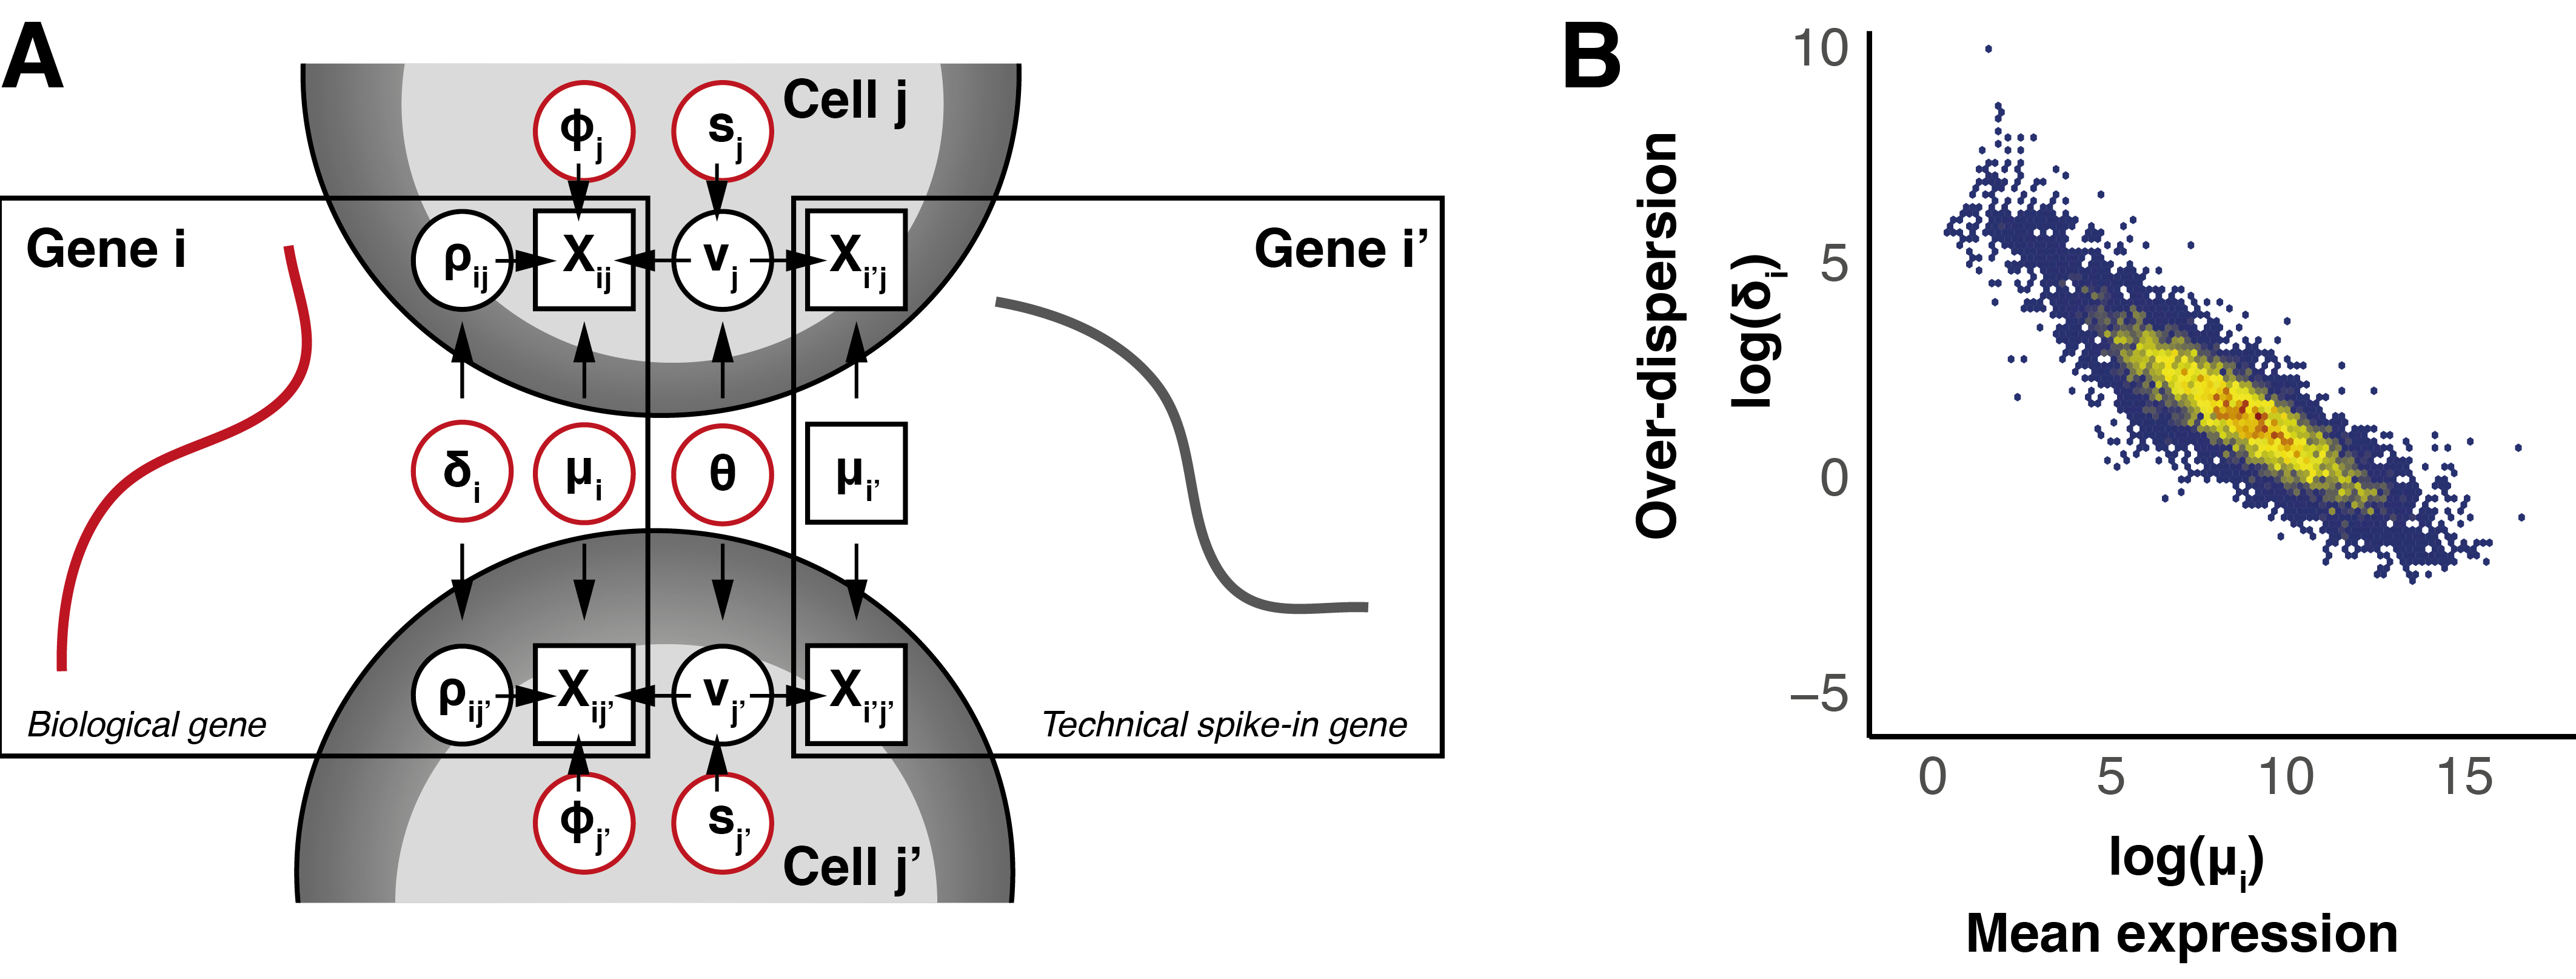
\includegraphics[width=\textwidth]{Fig_19.png}
\caption[The BASiCS model]{\textbf{The BASiCS model.}\\
\textbf{(A)} Hierarchical formulation of the negative-binomial model underlying BASiCS visualised for two cells (j and j') and two genes (i and i', gene i' represents a technical spike-in gene). Squared nodes indicate known quantities (observed expression counts and added number of spike-in molecules). Round nodes indicate unknown quantities. Red circles represent unknown model-parameters while black circles indicate the random effects that play intermediate roles effecting expression counts. Adapted from \citep{Vallejos2015BASiCS}, \textbf{(B)} Illustration of the typical confounding effect that is observed between gene-specific estimates of over-dispersion parameters $\delta_i$ and mean expression parameters $\mu_i$.}
\label{fig0:BASiCS}
\end{figure}


Given the NB model, the expected biological counts take the form:

\begin{equation}
\mathbb{E}(X_{ij}|\mu_i,\delta_i,\phi_j,s_j,\theta)=\phi_js_j\mu_i
\end{equation}

This formulation can be used to obtain normalized counts. Furthermore, the coefficient of variation is defined as:

\begin{equation}
\textnormal{CV}^2(X_{ij}|\mu_i,\delta_i,\phi_j,s_j,\theta)=\frac{1}{\phi_js_j\mu_i} + \theta + \delta_i(\theta + 1)
\end{equation}

As discussed in Vallejos \emph{et al.}, 2016 \citep{Vallejos2016}, the CV$^2$ is inversely proportional to the mean expression $\mu_i$. Furthermore, $\delta_i$ can be interpreted as the residual CV$^2$ after removing Poisson sampling and residual technical over-dispersion \citep{Vallejos2015BASiCS, Vallejos2016}. We will therefore use $\delta_i$ as a proxy for the biological part of transcriptional variability when modelling scRNA-Seq data.\\

Posterior inference is implemented using adaptive Metropolis-within-Gibbs sampling (see section \ref{sec0:posterior_inference}) \citep{Vallejos2015BASiCS, Vallejos2016}. Once posterior distributions are obtained, down-stream analyses can be performed. These include: normalisation of expression counts, variance decomposition into biological and technical noise, detection of highly and lowly variable genes and differential mean and differential over-dispersion testing. The later is done by computing the tail posterior probabilities of the difference in mean expression or over-dispersion between two conditions ($p$ and $p'$) is larger than an evidence threshold $\tau_0$ or $\omega_0$ (see section \ref{sec0:decision}, and \citep{Bochkina2007, Vallejos2016}):

\begin{align*}
\pi_{ipp'}(\tau_0)&\equiv{}P(|log(\mu_i^{(p)}/\mu_i^{(p')})|>\tau_0|D)>\alpha_m\\
\pi_{ipp'}(\omega_0)&\equiv{}P(|log(\delta_i^{(p)}/\delta_i^{(p')})|>\omega_0|D)>\alpha_d
\end{align*}

If the tail posterior probability is larger than a given propability threshold $\alpha_m$ or $\alpha_d$, the gene is considered to be differentially expressed or differentially over-dispersed \citep{Vallejos2016}. The evidence threshold is usually fixed \emph{a priori} and the probability threshold is defined to control the expected false discovery rate (EFDR) to (e.g.) 5\% \cite{Newton2004, Vallejos2016}.\\

As in Vallejos \emph{et al.}, 2016 \citep{Vallejos2016}, estimates of the over-dispersion parameters $\delta$ are negatively correlated to mean expression $\mu$ \textbf{(Fig.~\ref{fig0:BASiCS}B)}. This indicates that in homogeneous populations of cells, highly expressed genes tend to be less noisy than lowly expressed genes. This effect confounds differential over-dispersion testing when mean expression changes. Therefore, when assessing changes in over-dispersion, only genes with no changes in mean expression are considered (see Vallejos \emph{et al.}, 2016 \citep{Vallejos2016}, section \ref{sec1:varaibility} and \textbf{Box 2}).  

\subsection{Scalability of Bayesian inference}

With the development of droplet based scRNA-Seq approaches \citep{Macosko2015, Klein2015} and large scale microwell techniques \citep{Han2018}, the amount of cells that can be assayed in one experiment scaled from hundreds to hundreds of thousands \citep{Svensson2018}. To learn model parameters of a generative model across all cells and all genes became computationally challenging when considering a full Bayesian MCMC based approach. To address this problem, a model framework called single-cell variational inference (scVI) has been developed that uses stochastic optimization within a variational autoencoder network to approximate posterior distributions of model parameters and latent factors \citep{Lopez2018}. In scVI transcriptomes of each cell are encoded through a non-linear transformation into a low-dimensional latent vector of normal random variables. 

\newpage

\begin{wrapfigure}{r}{0.5\textwidth}
\centering    
\includegraphics[width=0.48\textwidth]{Fig_20.png}
\caption[The scVI model.]{\textbf{The scVI model.} \\
Hierarchical representation of the scVI model. Shaded nodes indicate observed quantities. White nodes indicated latent random variables. Shaded diamonds represent constants which were set \emph{a priori}. White diamonds indicate variables shared across all genes and all cells. Edges show conditional dependency. Adapted from \citep{Lopez2018}.}
\label{fig0:constrains}
\vspace{-60mm}
\end{wrapfigure}

The latent representation is non-linearly transformed to generate a posterior distribution of model parameters based on a zero-inflated negative binomial model. For this, the transcript count $x_{n,g}$ of gene $g$ in cell $n$ is modelled as:

\begin{align*}
x_{n,g} & = 
 \left\lbrace
  \begin{aligned}
    & y_{n,g} && \textnormal{if} \; h_{n,g} = 0,  \\ 
    & 0 && \textnormal{otherwise}    	    
  \end{aligned}
\right.\\
h_{n,g} & \sim \textnormal{Bernoulli}(f_h^g(z_n,s_n))\\
y_{n,g} & \sim \textnormal{Poisson}(l_nw_{n.g})\\
w_{n,g} & \sim \textnormal{Gamma}(\rho^g_n, \theta)\\
\rho_n & = f_w(z_n,s_n)\\
l_n & \sim \textnormal{log-Normal}(l_{\mu},l^2_{\sigma})\\
z_n & \sim \textnormal{Normal}(0,I)
\end{align*}

\vspace{1cm}

In this model, the negative binomial distribution is realized as a hierarchical formulation of $y_{n,g}$ being Poisson distributed around the latent random variable $l_n$ with an additional random effect $w_{n,g}$. Additionally, the zero-inflation of the model is controlled by the latent variable $h_{n,g}$. $l_n$ is a random variable that represents nuisance variation due to differences in capture efficiency and sequencing depth and correlates with log-library size. $l_n$ is log-normal distributed parametrized by $l_\mu,l_\sigma\in\mathbb{R}^B_+$ which are empirical mean and variance estimates of the log-library size per batch in $B$ and which are therefore constants in the model \textbf{(Fig.~\ref{fig0:scVI}A)}.\\

$w_{n,g}$ is Gamma distributed with the shape parameter $\rho_n^g$ and the scale parameter $\theta$. $\rho_g$ represents an intermediate matrix that relates the observations $x_{n,g}$ to the latent variables $z_n$. It provides a batch-corrected, normalized estimate of the percentage of transcripts in each cell $n$ from each gene $g$. $\theta$ is a global inverse-dispersion variable shared across all genes and all cells. The latent variable $z_n$ captures a latent representation of the data reflecting biological variation between the cells. $f_w$ and $f_h$ are neural networks mapping the latent space and batch annotation back to the full dimension of all genes: $\mathbb{R}^d\times{}\left\lbrace0,1\right\rbrace^B\rightarrow\mathbb{R}^G$.\\

Fast inference of this model is implemented via stochastic optimization. First, the latent variables $w_{n,g}$, $h_{n,g}$ and $y_{n,g}$ are integrated out by controlling that $p(x_{n,g}|z_n,l_n,s_n)$ has a closed form density and is zero-inflated negative binomial (see Appendix A in \citep{Lopez2018}). In this formulation, the distribution of $x_{n,g}$ is only conditioned on the latent variables $z_n$ and $l_n$. The posterior distributions has therefore the following form: $p(z_n,l_n|x_{n,g},s_n)$. Mean-field variational inference is used to parameterized the posterior as:

\begin{equation}
p(z_n,l_n|x_{n,g},s_n)=p(z_n|x_{n,g},s_n)p(l_n|x_{n,g},s_n)
\end{equation} 

The variational distribution $q(z_n|\cdot)$ is chosen to be Gaussian with diagonal covariance matrix and mean and covariance are learned by a multilayer perceptron (MLP) network similar to Kingma \emph{et al.}, 2013 \citep{Kingma2013}. Similarly, $q(l_n|\cdot)$ is chosen to be log-normal where the scalar mean and variance are learned by a MLP \citep{Kingma2013}.The authors found used reparametrization to solve the variational lower bound of this system \cite{Lopez2018, Kingma2013}. Furthermore, scVI uses stochastic optimization by sampling 128 cells for optimizing the objective function. This approach is therefore fast (5 hours for > 1 million cells and 750 genes and 10 hours for > 1 million cells and 10,000 genes) and memory efficient. \\

The authors concluded that: 1. scRNA-Seq data is better fitted with a ZINB than log-Normal or zero-inflated log-Norm; 2. Zero-inflation is not needed as part of the model since the zeros in dataset can be explained by NB distribution; 3. When the number of cells is smaller than number of genes, scVI underfits the data \citep{Lopez2018}. The clear strength of the model is the fast estimation of model parameters that can be used for down-stream analysis (e.g. visualization, normalization, differential expression testing)
 

